%==========================================================================================
\section{ Methods }

The hardware, coordinate frames, and algorithms used are discussed in this section.

%-----------------------------------------------------------------------------------
\subsection{ Hardware }

 This project implements SLAM on a real hexapod robot platform. This platform is built of discrete components, including the hexapod hardware, sensors, and processors.

%------------------------------------------------
\subsubsection{ Hexapod }

This project uses the Freenove Big Hexapod kit as the hardware base. This kit comes with a six-legged robot chassis, where each leg has three degrees of freedom (DOF) that can be individually controlled. Each joint is actuated by an individual MG-996R servo motor, which can be commanded to move between $0-180^{\degree}$ given a 50 Hz pulse width modulation (PWM) signal. To manage communication to all 18 leg servos, the servos are controlled by the PCA9685 servo driver module, which has a standard Python library to allow software control of the PWM signals.

%------------------------------------------------
\subsubsection{ Processor }
The Raspberry Pi (RPi) 4 acts as the main processor of the robot assembly.  The RPi's CPU is a Broadcom BCM2711B0 with stock clock speeds of 1.5GHz, which has been over-clocked to 1.9 GHz for improved performance.  The model RPi used in this project includes 8MB of DDR RAM. A heat sink and active fan are used to keep CPU temperatures manageable during strenuous processing. The RPi is also setup to boot from an external SSD connected through USB 3.0, rather than the typical SD card boot hardware; this improves read-write speed and boot times.

\begin{figure}[H]
    \centerline{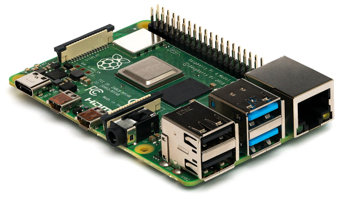
\includegraphics[scale=0.8]{figures/pi1.png}}
    \caption{The Raspberry Pi 4 single-board computer}
    \label{fig:raspberry_pi}
\end{figure}

%------------------------------------------------
\subsubsection{ Seeker Gimble }

The Freenove Big Hexapod kit comes equipped with two additional sensors used for this project: an ultrasonic range sensor and a camera. These sensors are mounted together on a two-axis gimble called the ``seeker.'' The seeker can be pointed in azimuth and elevation directions individually by two MG90S servo motors, which are controlled by the RPi similar to the leg servos.

%------------------------------------------------
\subsubsection{ Raspberry Pi Camera Module}

A Raspberry Pi OV5647 infared night vision camera module is mounted to the seeker and is optimized for use with the Raspberry Pi.  It connects via a dedicated ``camera module port'' on the RPi's PCBA. It can be used for both still photos and video, and is the primary sensor for this project.

\begin{figure}[h]
    \centering
    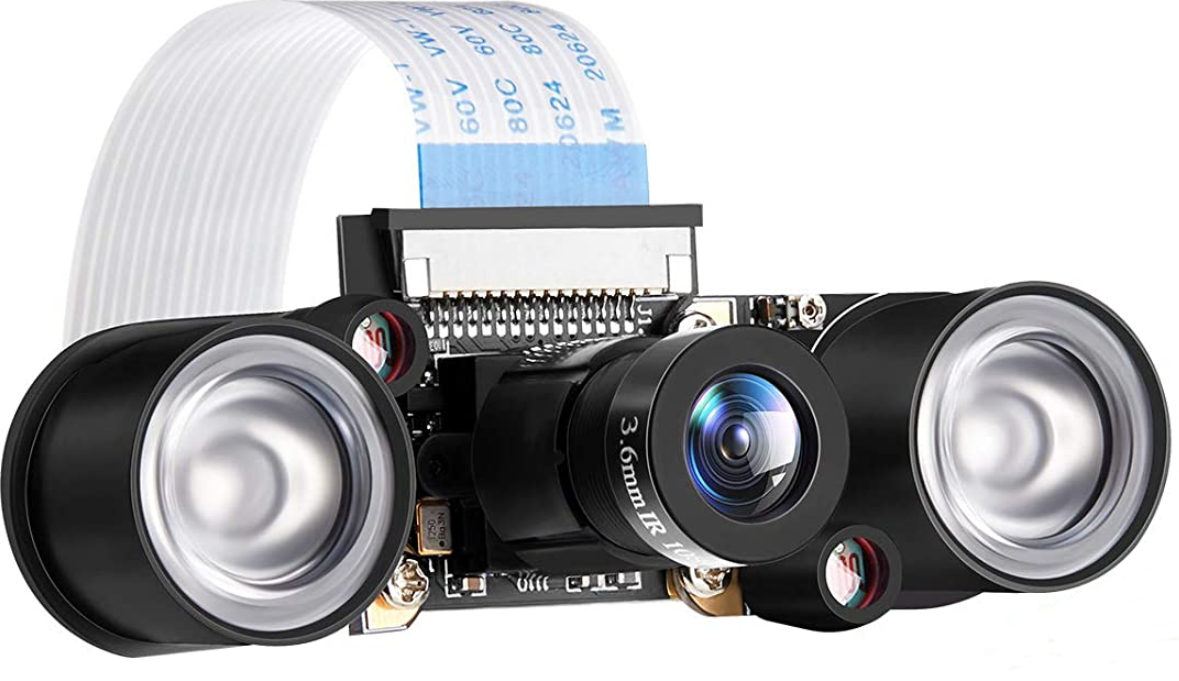
\includegraphics[scale=0.15]{figures/camera.png}
    \caption{Raspberry Pi OV5647 infared nigh vision camera module}
    \label{fig:raspberry_pi_cam}
\end{figure}

%------------------------------------------------
\subsubsection{ Inertial Measurement Unit (IMU)}
The MPU-6050 is an affordable, OTS inertial measurement unit (IMU) that is capable of providing linear acceleration, angular velocity, and temperature measurements to the Raspberry Pi at 50 Hz \cite{mpu6050}.  The IMU is hard-mounted to the motor driver board and is located just underneath the RPi. The IMU connects to the RPi via I\textsuperscript{2}C on the RPi's GPIO module.

This low-cost IMU presents inconsistent bias values for each signal which must be removed to prevent pose estimation drift. To perform this, a calibration routine was implemented in the IMU node at initialization, which assumes the robot body is static and level with the ground. The sensor is polled for some fixed time period (0.5s), and an average of all readings from both the accelerometer and gyroscope is computed. Gravitational acceleration of $9.81 m/s^2$ is removed from the $\hat{z}$ component of the accelerometer. These bias values are then removed from all future IMU measurements before publishing the data out as a ROS topic.

%------------------------------------------------
\subsubsection{ Desktop Computer }
To aleviate the computational burden of ORB-SLAM3 on the RPi, the distributed processing capabilities of ROS1 were exploited for this project by using a desktop computer to supplement the processing. This computer contained an AMD Ryzen 7 3800X 8-core CPU, an Nvidia RTX 2060 Super graphics processor, and 32Gb of onboard RAM running Ubuntu 20.04. The RPi ran all hardware-dependent ROS nodes, including the camera and IMU sensor nodes and the servo actuator nodes. All other ROS nodes, the ROS core, and any extra analysis tools, were run on the desktop machine. Communication was handled wirelessly using the local network WiFi.

%------------------------------------------------
\subsection{ Sensor Calibration }
To effectively use the sensors, they first needed to be calibrated. The approaches used are discussed below.

\subsubsection{ Camera }
To calibrate the embedded camera with intrinsic hardware parameters, the open-source camera\_calibration ROS package was used \cite{cameracalibration}. This package contains a ROS node that subscribes to a camera video topic of type sensor\_msgs/Image \cite{imagemsg}. Users present a grid of known shape and dimension to the camera at different poses across the whole image field of view, as seen in Figure \ref{fig:camera_calibrate}. Once enough data is collected, the tool runs an optimization routine to calculate camera properties like focal length and distortion characteristics.

\begin{figure}[H]
    \centerline{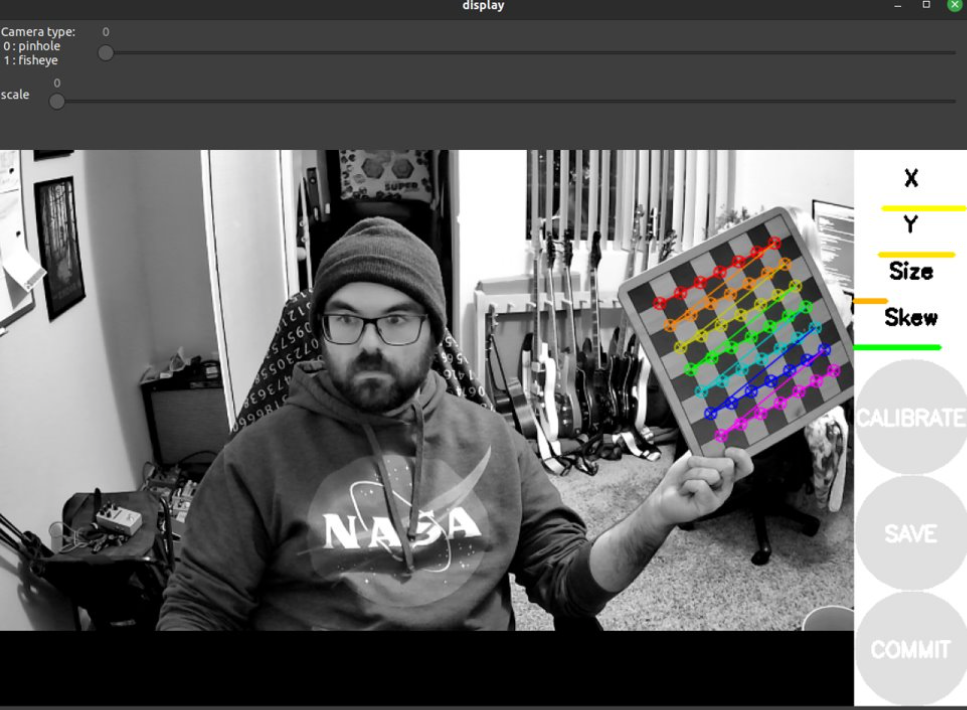
\includegraphics[scale=0.27]{figures/camera_calibrate.png}}
    \caption{ camera\_calibration GUI detecting a 7x7 checkerboard grid of known dimensions}
    \label{fig:camera_calibrate}
\end{figure}


%-----------------------------------------------------------------------------------
\subsection{ Coordinate Frames }

Several right-handed coordinate frames are defined and used throughout this project:

\begin{itemize}
    \item The odometry frame is used as the world-fixed coordinate frame. Both the extended Kalman filter (EKF) and the ORB\_SLAM3 algorithm estimate pose relative to this frame.

    \item The ground frame is placed under the robot body frame and is a child of the odometry frame. Desired foot positions for the walking gait are calculated in this frame, since motion is dependant on foot contact with the ground rather than relative to the robot body.

    \item The robot body frame is static relative to the hexapod chassis hardware and is referenced relative to the ground frame. The $\hat{x}_b$ direction points forward, the $\hat{y}_b$ direction points left (port side) of the body, and the $\hat{z}_b$ direction points straight up. This coordinate frame is located in the center of the robot belly such that this frame contacts and is parallel to the ground when $z_b = 0$.

    \item The seeker frame is kinematically linked to the body via a two axis gimble, with the $\hat{x}$ direction pointing out from the seeker. The camera is statically mounted on the seeker, with its own coordinate frame whos $\hat{z}$ direction points out from the seeker and the $\hat{x}$ direction points to the robot starboard side. The transformation from body to camera frame is a function of seeker azimuth and elevation servo angles. Because the seeker gimble servos do not give encoder data back to the RPi, it is assumed that commanded joint angles are the true joint angles. This transformation is calculated as follows.

    \[
    T^b_c = T^b_n T^n_{az} T^{az}_{el} T^{el}_{c}
    \]

    \[
    T^b_n = \begin{bmatrix} 0 & -1 & 0 & 0 \\
                            1 & 0 & 0 & 0.0762 \\
                            0 & 0 & 1 & 0.1386 \\
                            0 & 0 & 0 & 1 \end{bmatrix}
    \]
    \[
    T^n_{az} = \begin{bmatrix} \cos{az} & 0 & \sin{az} & 0 \\
                               \sin{az} & 0 & -\cos{az} & 0 \\
                               0 & 1 & 0 & 0 \\
                               0 & 0 & 0 & 1 \end{bmatrix}
    \]
    \[
    T^{az}_{el} = \begin{bmatrix} \cos{el} & 0 & -\sin{el} & L \cos{el} \\
                                  \sin{el} & 0 & \cos{el} & L \sin{el} \\
                                  0 & -1 & 0 & 0 \\
                                  0 & 0 & 0 & 1\end{bmatrix}
    \]

    \[
    T^{el}_{c} = \begin{bmatrix} 0 &  0 & 1 & 0 \\
                                 0 & -1 & 0 & 0.0167 \\
                                 1 &  0 & 0 & 0 \\
                                 0 &  0 & 0 & 1 \end{bmatrix}
    \]

Where $L$ is the length of the gimble, and $az$ and $el$ are the azimuth and elevation angles, respectively. All angles are given in radians, and distance is given in meters.

\end{itemize}

\begin{figure}[h]
    \centering
    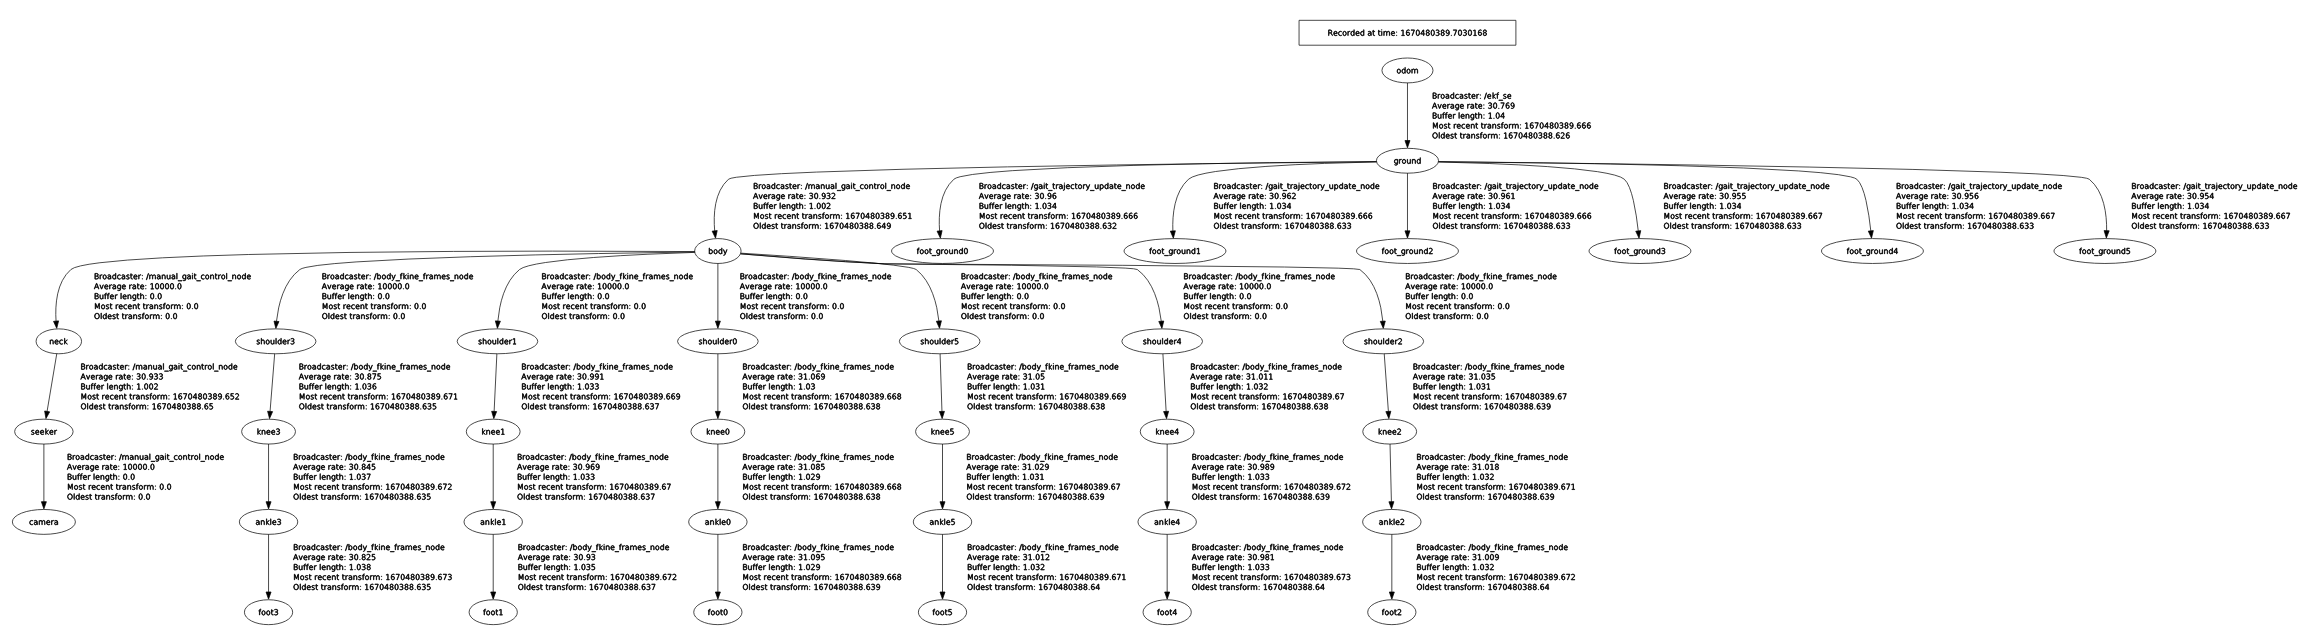
\includegraphics[scale=0.11]{figures/tf_tree.png}
    \caption{ ROS tf2 \cite{tf2} kinematic transformation tree, including all leg-related frames }
    \label{fig:tf_tree}
\end{figure}

%-----------------------------------------------------------------------------------
\subsection{ Software Architecture }

The RPi embedded on the robot runs Ubuntu Mate 20.04 as the operating system. All control software for the robot is written as ROS1 Noetic nodes, written in Python and C++. Nodes are broken up between hardware control, gait manipulation, and analytical or sensor processing. An RQT ROS node graph can be seen in Figure \ref{fig:rqt}.


\begin{figure}[h]
    \centering
    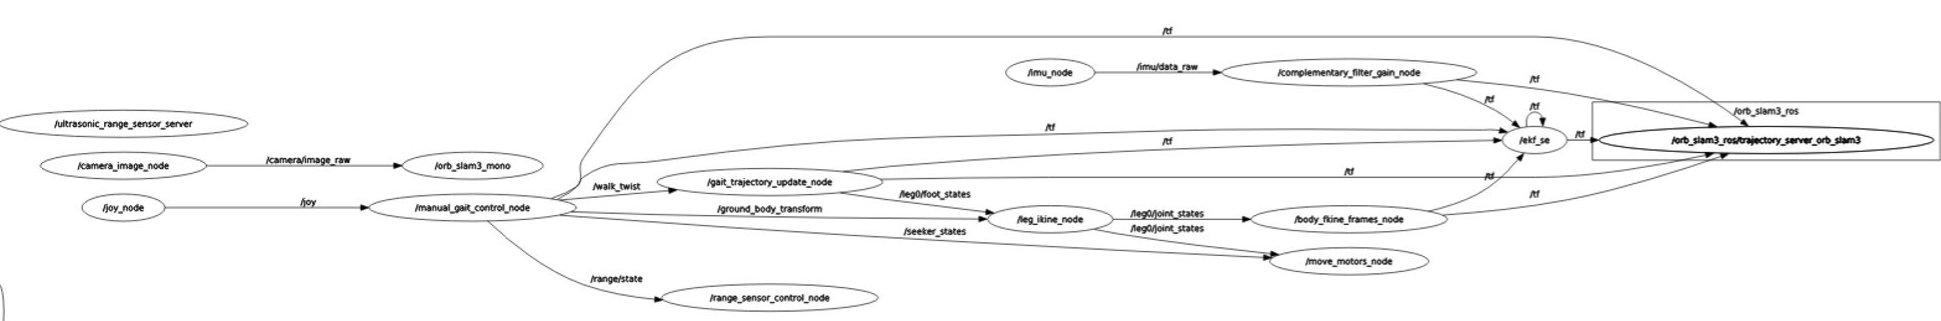
\includegraphics[scale=0.12]{figures/rosgraph.png}
    \caption{ Node design for ROS software architecture }
    \label{fig:rqt}
\end{figure}

In order to facilitation motion through the space we wish to map, a master controller node receives input from an Xbox controller to determine the desired body motion. This node outputs a twist vector and a body pose relative to the ground, as well as seeker gimble angles. The gait update node receives the twist vector and calculates new desired foot positions. An inverse kinematics node then calculates new joint angles, which are received by the motor driver node to actuate the servo motors.

\subsubsection{ Extended Kalman Filter (EKF)}

For continuous body pose estimation, the robot\_localization ROS package \cite{robotlocalization} was used to implement an extended Kalman filter (EKF). This filter receives the commanded twist vector in the ground frame, as well as IMU sensor data in the body frame, and estimates the robot's pose relative to the fixed odometry frame over time.

\subsubsection{ ORB-SLAM3 Node}

A fork of the ORB-SLAM3 library was used for this project \cite{orb_slam_ros}. This package modifies the original ORB-SLAM3 library to streamline interfacing it with ROS1 Noetic. An additional ROS wrapper repository was also used to call the ORB-SLAM3 algorithm as a ROS node \cite{orb_slam_ros_wrapper}. This wrapper was modified for this project to publish the camera pose as a ROS PoseStamped messages \cite{posestamped} and the map as a ROS PointCloud2 message \cite{pointcloud2} when the algorithm maintains a track on the map. The node accpets a configuration YAML file with parameters, including the calibrated camera properties, camera framerate, and internal settings for the ORB-SLAM3 algorithm. This node subscribes to the camera data published by the robot.
